%%
%% Copyright 2007, 2008, 2009 Elsevier Ltd
%%
%% This file is part of the 'Elsarticle Bundle'.
%% ---------------------------------------------
%%
%% It may be distributed under the conditions of the LaTeX Project Public
%% License, either version 1.2 of this license or (at your option) any
%% later version.  The latest version of this license is in
%%    http://www.latex-project.org/lppl.txt
%% and version 1.2 or later is part of all distributions of LaTeX
%% version 1999/12/01 or later.
%%
%% The list of all files belonging to the 'Elsarticle Bundle' is
%% given in the file `manifest.txt'.
%%

%% Template article for Elsevier's document class `elsarticle'
%% with numbered style bibliographic references
%% SP 2008/03/01
%%
%%
%%
%% $Id: elsarticle-template-num.tex 4 2009-10-24 08:22:58Z rishi $
%%
%%
\documentclass[preprint,12pt,3p]{elsarticle}

%% Use the option review to obtain double line spacing
%% \documentclass[preprint,review,12pt]{elsarticle}

%% Use the options 1p,twocolumn; 3p; 3p,twocolumn; 5p; or 5p,twocolumn
%% for a journal layout:
%% \documentclass[final,1p,times]{elsarticle}
%% \documentclass[final,1p,times,twocolumn]{elsarticle}
%% \documentclass[final,3p,times]{elsarticle}
%% \documentclass[final,3p,times,twocolumn]{elsarticle}
%% \documentclass[final,5p,times]{elsarticle}
%% \documentclass[final,5p,times,twocolumn]{elsarticle}

%% if you use PostScript figures in your article
%% use the graphics package for simple commands
%% \usepackage{graphics}
%% or use the graphicx package for more complicated commands
%% \usepackage{graphicx}
%% or use the epsfig package if you prefer to use the old commands
%% \usepackage{epsfig}

%% The amssymb package provides various useful mathematical symbols
\usepackage{amssymb}
%% The amsthm package provides extended theorem environments
%% \usepackage{amsthm}

%% The lineno packages adds line numbers. Start line numbering with
%% \begin{linenumbers}, end it with \end{linenumbers}. Or switch it on
%% for the whole article with \linenumbers after \end{frontmatter}.
\usepackage{lineno}

%% natbib.sty is loaded by default. However, natbib options can be
%% provided with \biboptions{...} command. Following options are
%% valid:

%%   round  -  round parentheses are used (default)
%%   square -  square brackets are used   [option]
%%   curly  -  curly braces are used      {option}
%%   angle  -  angle brackets are used    <option>
%%   semicolon  -  multiple citations separated by semi-colon
%%   colon  - same as semicolon, an earlier confusion
%%   comma  -  separated by comma
%%   numbers-  selects numerical citations
%%   super  -  numerical citations as superscripts
%%   sort   -  sorts multiple citations according to order in ref. list
%%   sort&compress   -  like sort, but also compresses numerical citations
%%   compress - compresses without sorting
%%
%% \biboptions{comma,round}

% \biboptions{}

%Todd added this for strikeout \sout{}
\usepackage[normalem]{ulem}
%Todd added this for the reference to essence.sv.cmu.edu
\usepackage{hyperref}
%Todd added this to fix tables with an H
\usepackage{float}


\journal{Todd Sedano's ECE Prospectus Committee}

\begin{document}

\begin{frontmatter}

\title{Empirical Study of Iterative Software Development in Academia and Industry: Effectiveness, Optimization, and Extension of the Essence Kernel}

\author{Todd Sedano}
\ead{professor@gmail.com}

% \author{C\'ecile P\'eraire}
% \ead{cecile.peraire@sv.cmu.edu}

\address{Carnegie Mellon University}
\address{Silicon Valley Campus}
\address{Moffett Field, CA 94035, USA}


\begin{abstract}
Software development continues to be a complex endeavor involving many disciplines and skill sets. Practitioners and researchers experiment, research, and adopt practices to simplify, understand, and create effective processes. 

Given the plethora of practices and methods, the Software Engineering Method and Theory (SEMAT) community created the Essence kernel as a unifying framework for describing and analyzing software engineering endeavors. 

My research goal is to evaluate the Essence kernel for practical use on academic and industrial software development projects, identify issues, and research solutions grounded in empirical evidence. 

At Carnegie Mellon University in Silicon Valley, I conducted a field study with masters of science in software engineering students as they completed team-based capstone projects using the Essence kernel. During weekly Essence Reflection meetings, the Essence kernel checklists helped students identify relevant goals to achieve, which enabled the team to steer the project to higher states. The student teams found value during project inception. However, teams found less value during the construction phase of iterative projects, as the Essence kernel offered few new goals hence loosing its ability to help the team steer the project. The original Essence kernel is method agnostic and does not directly support iterative development. Since most of agile software development occurs via iterative software development, adapting Essence kernel to have goals during iterative construction phase would increase its value to software development teams.

Following these results in academia, my objective is to continue my research in industry, with a focus on Pivotal. One of my next goals is to adapt the Essence kernel for use at Pivotal by providing a kernel extension that matches Pivotal's engineering experiences and practices. My plan is to conduct participant-observation of several software development projects at Pivotal. I will interview many software engineers and product managers to collect additional data. I'll iterate my research by incorporating this feedback. My expected results is a modified kernel or kernel extension grounded in empirical data that supports iterative software development. 

%I have demonstrated that generic algorithms can be used to create kernels from empirical data. I created the Partial Ordering fitness function for evaluating candidate kernels against empirical data. The research shows that alternative structures for the kernel are necessary to best reflect the data.

%I created a research tool.
\end{abstract}

\begin{keyword}
%% keywords here, in the form: keyword \sep keyword
Essence Kernel \sep Empirical Research \sep Iterative Software Development
%% MSC codes here, in the form: \MSC code \sep code
%% or \MSC[2008] code \sep code (2000 is the default)
\end{keyword}

\end{frontmatter}

%%
%% Start line numbering here if you want
%%
%%\linenumbers

\section{Introduction}

\subsection{Background}
Software engineers often struggle to effectively run software projects. Researchers and practitioners have examined ways to handle the ``software crisis" since as early as the first Nato Software Engineering Conference in 1968 \cite{Naur1969}. 

Engineers address the complexity of software development with practices and methods that guide the development process. Practices, such as formal code inspection, are specific and generally accepted activities performed by a practitioner to achieve desired outcomes. Methods, such as the Rational Unified Process (RUP), are a set of synergistic, cooperating practices combined with a lifecycle such as waterfall, iterative, or incremental. Methods guide most aspects of a project, from beginning to end.

Since the 1950's software engineers have been creating methods to help manage software projects. Mark Kennaley illustrates the rich history of methods \cite{SDLC, ValueStream} in Figure \ref{ModernSoftwareEngineeringHistory}. Even with the plethora of software practices and methods, there remains missing an underlying foundation.

\begin{figure}[h]\vspace*{4pt}
\centerline{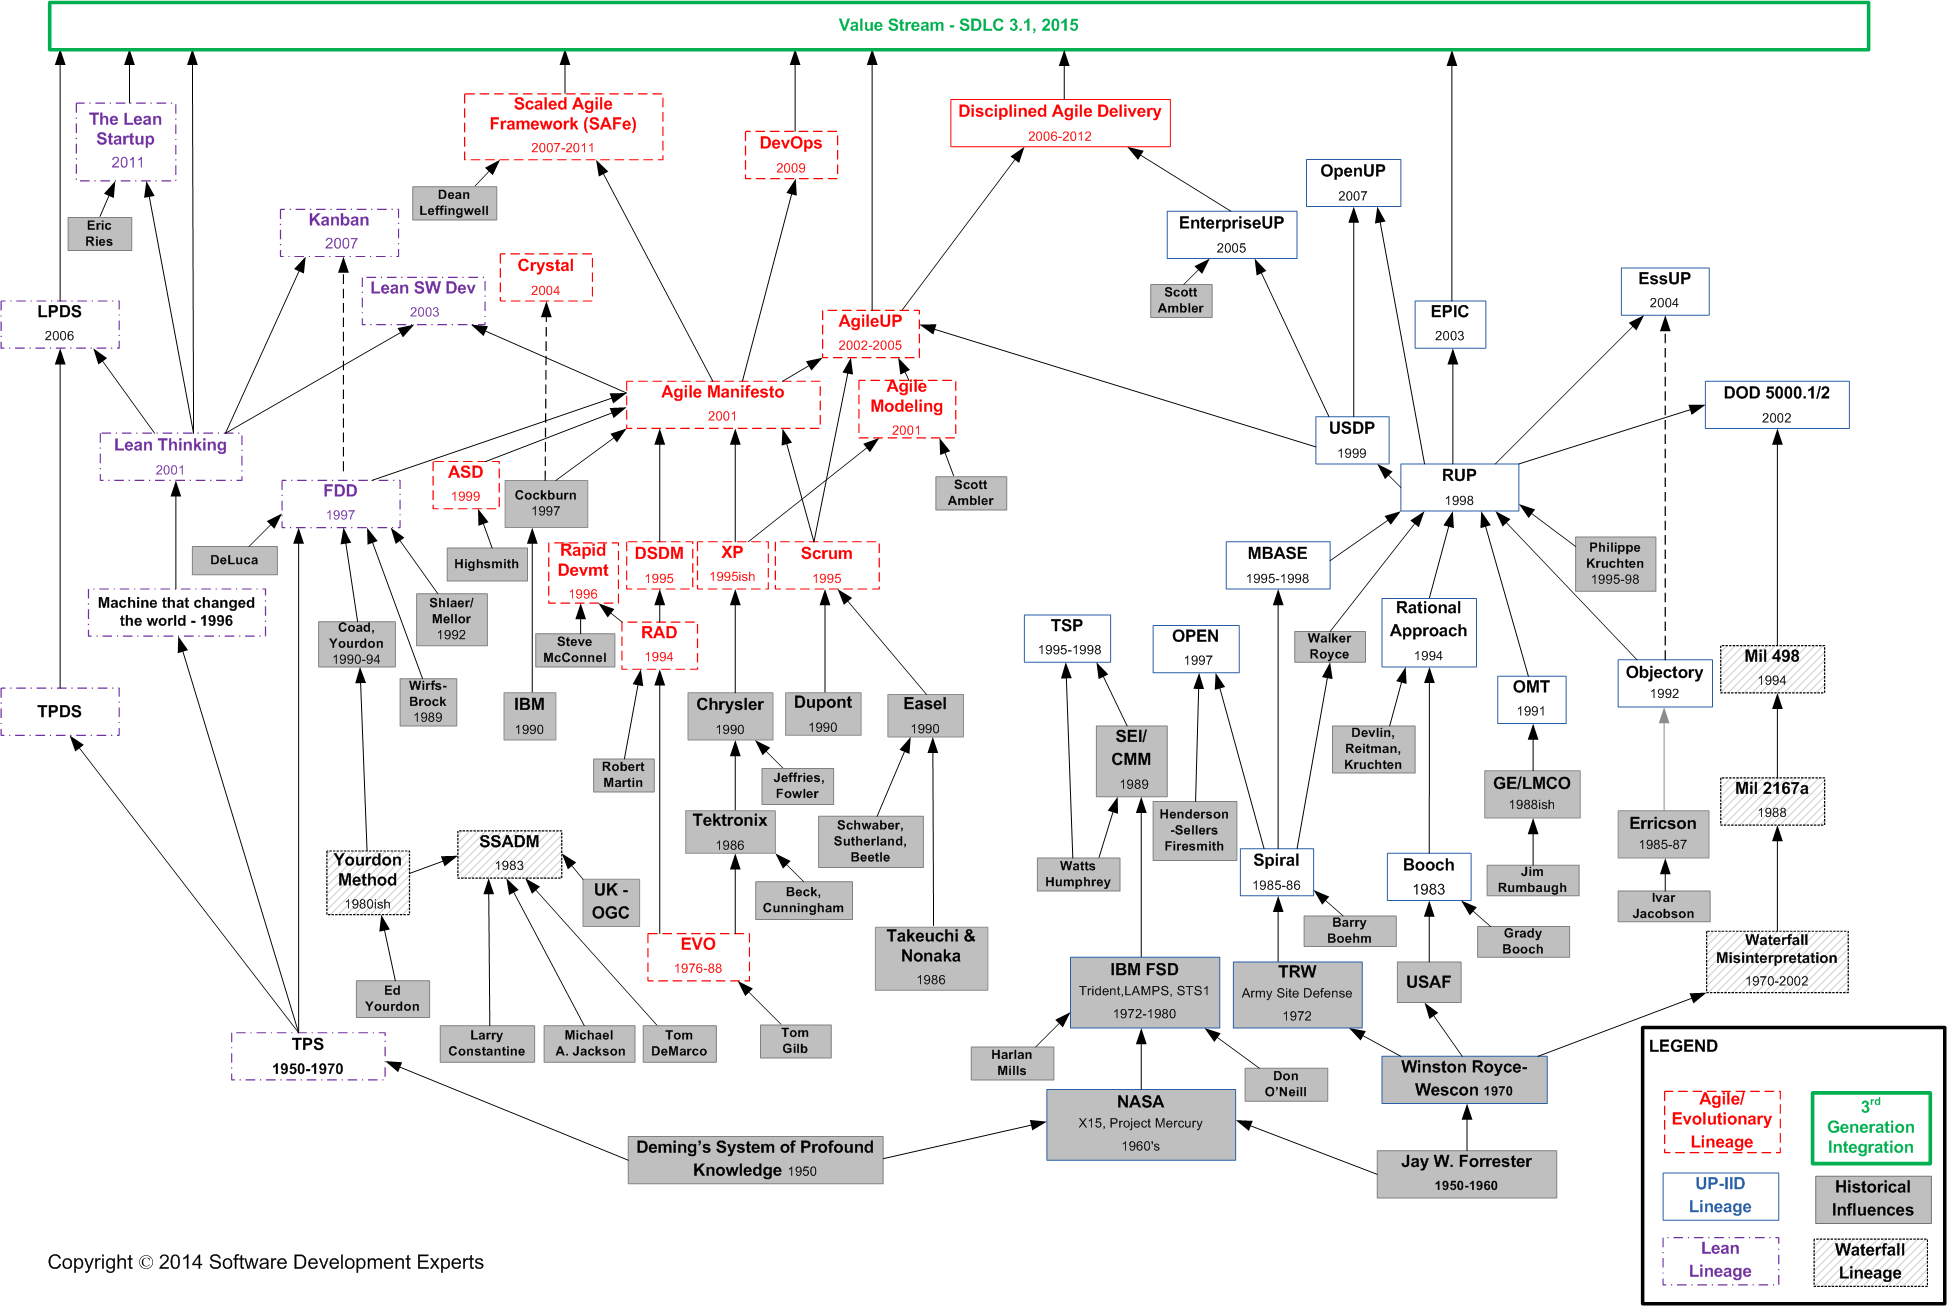
\includegraphics[width=6.4in]{field_study_images/ModernSoftwareEngineeringHistory}}
\caption{Evolution of Methods}\vspace*{-6pt}\label{ModernSoftwareEngineeringHistory}
\end{figure}

In response to this problem, the SEMAT community released the “Essence: Kernel and Language” as a potential unifying theory  ~\cite{OMGStandard}. The Essence kernel defines a set of dimensions, states, and checklists that are claimed to be "universal" and applicable to every software engineering project. The kernel aims at providing a “common ground” for all software development endeavors ~\cite{JacobsonQueue}. It should allow practitioners to map practices and methods to a set of common dimensions of software projects ~\cite{JacobsonQueue}.  It should assist any software development teams in monitoring their progress and steering their project throughout a project.

\subsection{Research Objective}
My research goal is to evaluate the Essence kernel for practical use on academic and industrial software development projects, identify issues, and research solutions grounded in empirical evidence.

\sout{The ``The Essence of Software Engineering: The SEMAT Kernel'' paper ~\cite{JacobsonQueue} describes the Essence kernel which allows practitioners to map practices and methods to a set of common dimensions of software projects. The framework consists of an Essence kernel containing ``universal" project dimensions, states, and checklists applicable to every software engineering project. Practices specific to certain circumstances are built on top of the kernel. Practices are then combined to define software development methods. The SEMAT community claims that Essence helps practitioners by providing a rigorous foundation and understanding for any software endeavor.  The “universal” Essence kernel aims at providing a “common ground” for all software development endeavors ~\cite{JacobsonQueue}. Software development teams can use Essence to monitor their progress and steer their project throughout a software project. }

My first goal is to evaluate the effectiveness of the Essence kernel monitoring and steering approach, and its applicability on a set of student and industry projects. Following recommendations for reporting research done in the empirical
software engineering community
\cite{GQM, Shaw}, I formed the
research goal using Goal/Question/Metric:
\cite{GQM}

\begin{table}[H]
\centering
\begin{tabular}{|p{2.00in}|p{4.10in}|}
\hline
Analyze & Essence kernel  \\ \hline
for the purpose of & evaluation \\ \hline
with respect to its & effectiveness \\ \hline
from the point of view of the & software development team and researcher \\ \hline
in the context of & software development in academia at Carnegie Mellon University in Silicon Valley and in industry at Pivotal. \\
\hline
\end{tabular}
\end{table}

Initial research performed in academia has demonstrated some issues with the kernel's effectiveness and applicability on iterative software projects. Therefore my next goal is to:

\begin{table}[H]
\centering
\begin{tabular}{|p{2.00in}|p{4.10in}|}
\hline
Analyze & iterative software projects  \\ \hline
for the purpose of & creating a kernel modification  \\ \hline
with respect to its & accuracy in describing empirical data \\ \hline
from the point of view of the & software development team and researcher \\ \hline
in the context of & software development in industry at Pivotal. \\
\hline
\end{tabular}
\end{table}

Creating a kernel modification from observations in industry could then be applied for team-based software courses in academia, and potentially improve the academic experience.

\subsection{Research Significance}

The Essence creators claim that Essence provides support to any software engineering project. Several authors have published papers explaining and promoting the Essence kernel \cite{CallToAction, JacobsonQueue, OMGStandard,  AgileSEMAT, EssenceBook, JacobsonMajorLeaugue, JacobsonNewSoftwareEngineering}. Essence kernel and language became an Object Management Group standard in 2014. Currently there is anecdotal evidence indicating that the Essence kernel adds value for software projects. My ICSE 2014 paper \cite{ICSE2014} documents empirical evidence that the Essence kernel does provide value in the context of master students working on a team-based capstone software project course. 
The paper also shows that the approach's ability to steer iterative projects is decreased during the construction phase of projects following an iterative lifecycle. Since iterative projects can spend the majority of their time in construction, discovering a solution to this problem would increase the value of the approach dramatically and make it relevant to a broader community including many software development teams working on iterative projects.

\subsection{Research Contributions and Plan}
% Here are some of my contributions so far:
% \begin{enumerate}
% \item I formalized project steering process based on the Essence kernel called Essence Reflection meetings \cite{};
% \item I evaluated Essence Reflection meetings against other Agile reflection meetings \cite{};
% \item  I utilized Essence Reflection meetings with software development teams to elicit the value of the Essence kernel for a student team-based project course \cite{};
% \item  I created a web-based tool to aid in data collection and running Essence Reflection meetings \cite{};
% \item I demonstrated a way to create and optimize alternative Essence kernels directly from empirical data \cite{};
% \item and I plan to create and evaluate a kernel extension for iterative software development in industry.
% \end{enumerate}   

I conducted a field study to identify the value in applying the Essence kernel in graduate software engineering program at Carnegie Mellon University in Silicon Valley. The field study revealed that the Essence kernel provides value to teams during project inception but does not reflect incremental progress achieved during construction on iterative projects. This work was presented at ICSE 2014 \cite{ICSE2014}. I summarize the field study's results in Section \ref{CMUFieldStudy}.

I define a process that leverages the Essence kernel to monitor students progress and steer their project in the context of team-based project courses. The process has been presented at conference workshops \cite{SCSE2015Tutorial, CSEET2015Workshop}. The process is based on Essence Reflection meetings where a facilitator guides a team through the Essence kernel for the purpose of project monitoring and steering. The Essence Reflection meeting process emerged from the field study. I compared and contrasted Essence Reflection meetings with other Agile reflection meetings. This work was presented at EASE 2014 \cite{EASE2014} and is summarized in Section \ref{EssenceReflectionMeetings}.

I created a web-based tool to guide development teams during Essence Reflection meetings, and to support my research by facilitating the collection of data related to the use of Essence by the teams throughout the project lifecycle. The tool is available at \url{http:\\esssence.sv.cmu.edu} and is described in Section \ref{EssenceTool}.

I programmed a genetic algorithm to utilize my collected empirical data to create random kernels, unlike the original kernel which is based on human experience and judgment. My research shows that kernels with smaller number of alphas result in higher fitness scores than the original kernel. Based on the analysis of the fitness function, a kernel with a fundamentally different structure might more effectively recommend next steps for a team during Essence Reflection meetings. I presented this work at SCSE 2015 and summarize it in Section \ref{KernelOptimization}.

Given that the Essence kernel does not reflect incremental progress achieved during construction on iterative projects, I plan to create a kernel extension or kernel replacement that supports iterative software development projects. I will use empirical data collected from field observations, participant-observation, and interviews of software teams in industry to derive an iterative kernel. Section \ref{PivotalKernelExtension} contains my research plan.

\section{Introduction to Essence}
\label{Method}

The SEMAT community created Essence as a universal framework for any software engineering project ~\cite{JacobsonQueue}. At the core of Essence is a ``kernel of widely-agreed elements'' built on an Essence Language shown in Figure \ref{EssenceLayers}. This general kernel can theoretically support any kind of software endeavor. A software project can define its software method by using the general kernel, extending the kernel, or defining additional practices on top of the kernel. Contrary to the kernel, practices are context dependent and may not be applicable to different situations. Software methods are compositions of practices that are known to work well together.

\begin{figure}[h]\vspace*{4pt}
\centerline{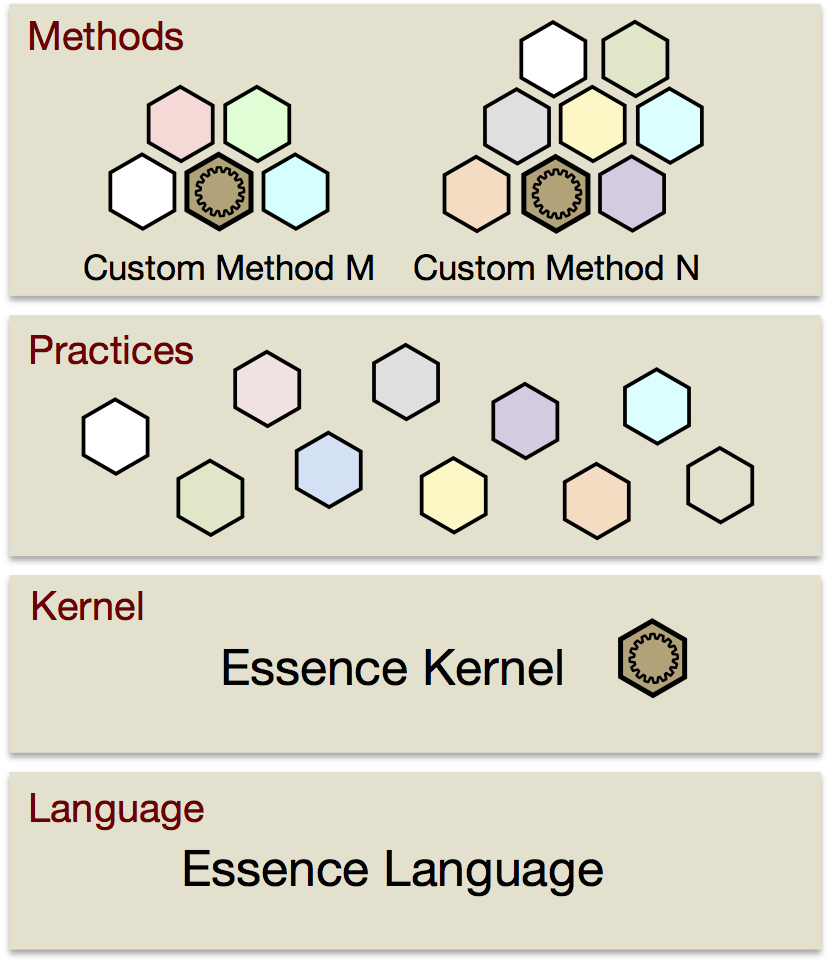
\includegraphics[width=2.2in]{kernel_images/EssenceLayers}}
\caption{Essence Method Architecture: Methods and Practices are Context Specific; the Kernel is Universal}\vspace*{-6pt}\label{EssenceLayers}
\end{figure}

The Essence kernel defines a ``universal'' characteristic or dimension of a software project as an ``alpha.'' The Essence kernel is composed of a set of alphas, alpha states, and alpha state checklist items. The seven alphas are \textbf{Stakeholders}, \textbf{Opportunity}, \textbf{Requirements}, \textbf{Software System}, \textbf{Team}, \textbf{Way of Working}, and \textbf{Work}. Essence decomposes each of these alphas into a set of states that represent a simple linear state machine as shown in Figure \ref{StateMachine}. For example, the \textbf{Requirements} alpha advances through the states \textit{Conceived}, \textit{Bounded}, \textit{Coherent}, \textit{Acceptable}, \textit{Addressed}, and \textit{Fulfilled.} Each state has a checklist or set of goals. To achieve a state, the project must satisfy every checklist item for that state \cite{OMGStandard}. If the project team knows the current state for each alpha, the team knows the overall project state, and which direction to take to get to the next project state.
 
\begin{figure}[h]\vspace*{4pt}
\centerline{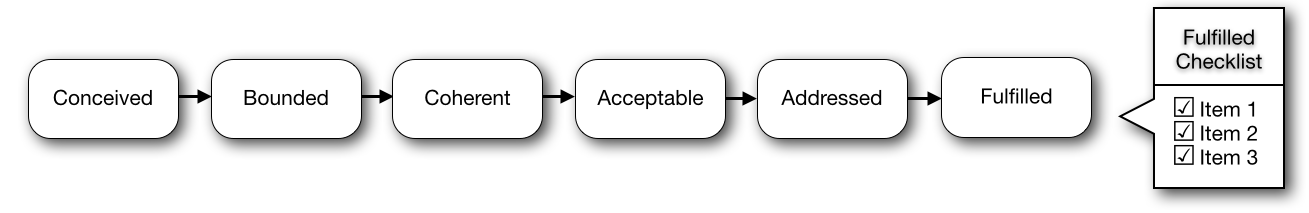
\includegraphics[width=5.4in]{kernel_images/StateMachineRequirements}}
\caption{Kernel's linear state machine for Requirements alpha (with Fulfilled checklist)}\vspace*{-6pt}\label{StateMachine}
\end{figure}

\section{Research Contributions}

\subsection{Kernel Evaluation in Academic Graduate Programs}
\label{CMUFieldStudy}
My research hypothesis contends that Essence's monitoring and steering approach provides a framework for students to look at their project holistically, helping them to address various project dimensions beyond implementation. I stipulate that the framework acts as a routine reminder about applicable software engineering practices covered in previous courses. For instance, by using this technique, I expected students to think about involving stakeholders, improving the team's way of working, and demonstrating that the software system has the desired quality characteristics.

The purpose of the field study \cite{ICSE2014} was to understand the value project teams receive from following the SEMAT Essence's monitoring and steering approach provided by the Essence kernel alphas and their states.  The two semester field study followed seven master of software engineering teams with no prior knowledge of Essence in a team-based capstone course called, ``Software Engineering Practicum." 

Each week a facilitator met with each team. The facilitator involvement was kept at a minimum to limit influencing the steering of the project. The role was constrained to guiding the team through the application of the Essence monitoring and steering approach, and to validating the objectivity of the team's self-assessment of their project state. By listening to the team's discussions, and asking clarification questions as needed, the facilitator gauged the project state. At times, this helped reduce the tendency of some teams to be overly pessimistic or optimistic about the project state. Qualitative and quantitative data was collected throughout the duration of the projects. Qualitative value was measured based on students' feedback collected mostly during the weekly Essence Reflection meetings, course reflection reports, and final survey. Quantitative value was measured based on alpha state progression as well as the number of work items generated during the weekly meetings and allowing bringing the project to a higher state.

I decomposed the research goal into four questions.

\textbf{Research Question 1: Does the Essence's monitoring and steering approach provide value to the project team?}

The field study showed that students received value from the approach provided by the kernel alphas and their states. In responding to a survey, 90\% of the students said that following the approach was worth their time (80\% of the students participated in the survey.) Similarly, 80\% said that they will use the approach on their next project. Most students have a positive perception of this approach as it helps them make decisions allowing to move their project forward. 

\textbf{Research Question 2: How does the approach provide value to the project team?}

The benefits that a project team received from the approach come primarily from the discussions that occur when the team is covering the various alphas. The discussions enabled the team to pause and assess the situation. The approach adds value by providing the project team with a holistic view of the project, a mechanism for monitoring progress and steering projects, as well as an effective structure for retrospective and risk management. This is provided in a simple, lightweight, non-prescriptive and method-agnostic fashion.

\textbf{Research Question 3: When in the project lifecycle does the approach add value?}

The value that the teams received from the approach varied over the project lifecycle. The study showed that most value is generated at the beginning of the project and that it decreases thereafter. Indeed, the approach gradually loses its ability to enable the team to steer the project by generating new work items leading to a higher project state as seen in Figure \ref{WorkItems}. However, most teams perceived value throughout the lifecycle from the approach's reflection mechanism.

\begin{figure}[h]\vspace*{4pt}
\centerline{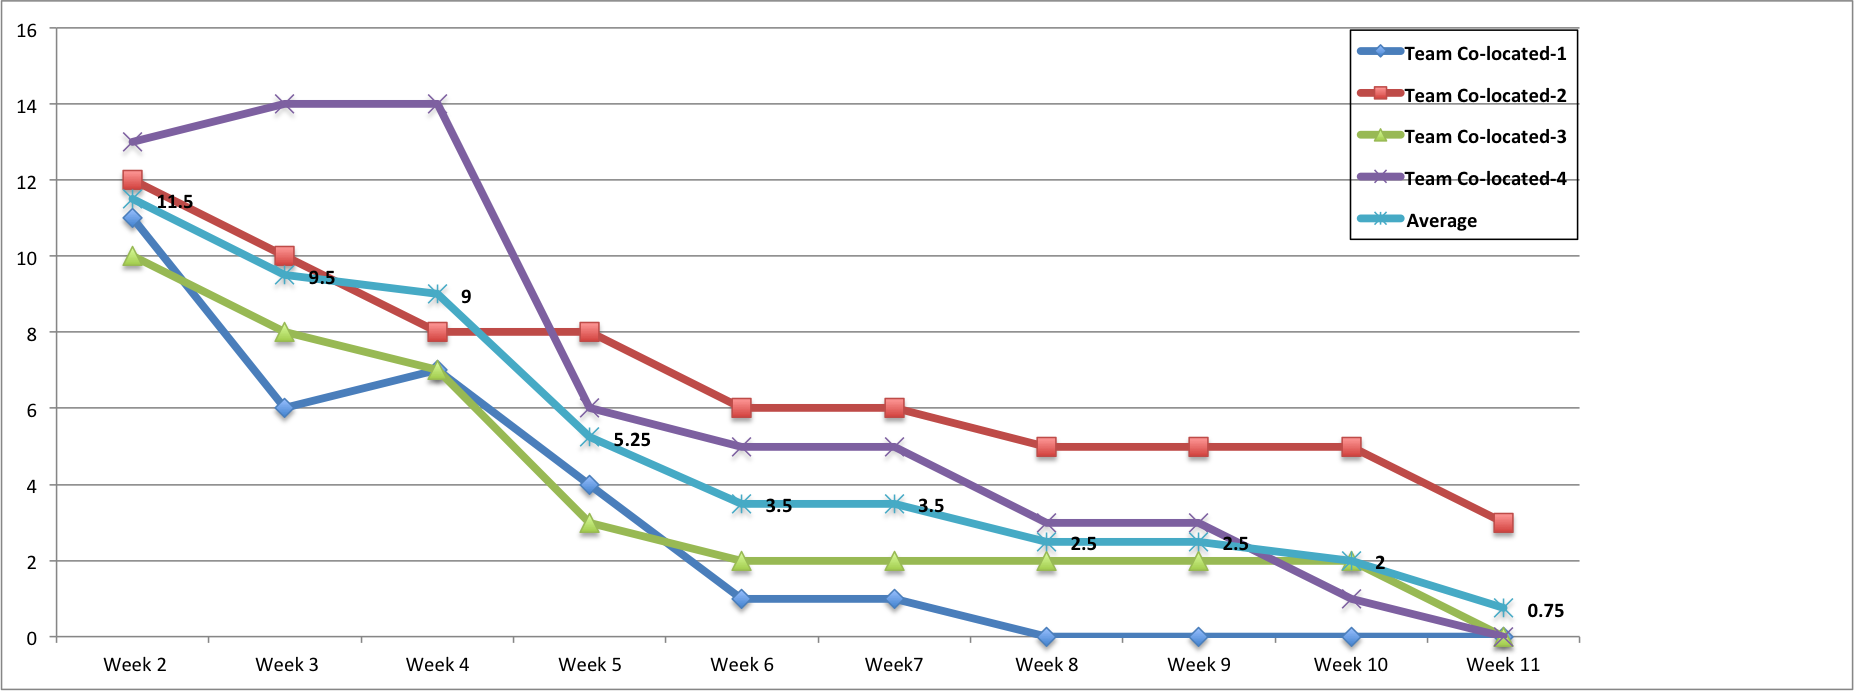
\includegraphics[width=5.4in]{field_study_images/WorkItems}}
\caption{Number of new work items generated per week}\vspace*{-6pt}\label{WorkItems}
\end{figure}

\textbf{Research Question 4: What are the limits of the approach and limitations to its effectiveness?}

The field study showed that the Essence framework does not reflect incremental progress achieved during the  construction phase on iterative projects. This is illustrated in Figure \ref{AlphaStateProgression}, showing a typical state progression of a team throughout the project. The initial state progression is driven by Essence-generated work items \sout{(shown in Figure \ref{WorkItems})}. However, during construction, the project reaches a stable state. The fact that the team is making incremental progress in each iteration is not captured by the model. 

\begin{figure}[h]\vspace*{4pt}
\centerline{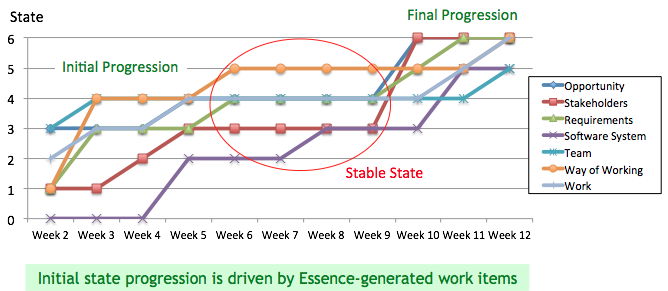
\includegraphics[width=5.4in]{field_study_images/AlphaStateProgression}}
\caption{Alpha state progression}\vspace*{-6pt}\label{AlphaStateProgression}
\end{figure}


This lack of steering support during construction on iterative projects is acceptable in the context of team-based project courses, where construction lasts only about a third of the project entire lifecyle. However, this could become a problem on longer iterative projects in industry, when teams spend the majority of the time in construction

%The SEMAT Essence's monitoring and steering approach provided by the kernel alphas and their states is constrained by its universal definition. For instance, since the kernel is lifecycle-independent, it does not provide specific support for iterative development. Similarly, since the kernel alpha states and their checklist items are specified at the project or release level, the approach does not provide specific support for lower level work, like technical work done during an iteration. As a result, the approach is optimum during project initiation and for monitoring and steering the work done at the project or release level. Beyond that, the approach's value decreases as the inherent limits of the universal kernel are reached. Pushing the limits should come from adding practices on top of the kernel, or by extending or altering the kernel definition.

Overall, the field study showed that the Essence kernel provides project teams with a simple, lightweight, non-prescriptive and method-agnostic way to examine their projects holistically, structure team reflections, manage risks, monitor progress and steer their projects. Compared to the ten previous years, the faculty in charge of the practicum course noted that there was ``much better early project organization with a lot less floundering." Indeed, the approach enabled students to learn to steer projects effectively by addressing the various dimensions of software engineering.

%The field study showed that most of the value from the Essence kernel occurs during project startup and initiation and for monitoring and steering the work done at the project or release level \cite{ICSE2014}. Since the work is done at the project or release level, it could be qualified as ``universal" as it is generally common across projects. This confirms that the kernel provides an effective support for universal work. Support for non-universal technical work should come from additional practices added on top of the kernel, or by extending or altering the kernel definition.}

\subsection{Essence Reflection Meetings}
\label{EssenceReflectionMeetings}
I define a process that leverages the Essence kernel in the context of team-based project courses. The process is based on Essence Reflection meetings and supported by a tool presented in the next section. The process has been presented at conference workshops \cite{SCSE2015Tutorial, CSEET2015Workshop}. 

Essence Reflection meetings are an alternative to Agile retrospection or weekly status meetings. The EASE 2014 paper \cite{EASE2014} compares and contrasts Essence Reflection meetings to other types of team reflection meetings.

Essence Reflection meetings are held weekly to guide student teams during their projects. During an Essence Reflection meeting, the team systematically uses the Essence kernel to identify where they are in the project, identity next possible goals, and generate work items to achieve those goals, hence steering the project to higher states. 

% For each alpha, team members ...
% \begin{enumerate}
% \item Read the alpha's states and the state's checklists,
% \item Identify the team's current state,
%     \begin{itemize}
%     \item Individually and silently determine the current state.
%     \item When ready, everyone reveals their state at same time.
%     \item Discuss differences of opinion until agreement is reached.
%     \item Records the current state.
%     \end{itemize}
% \item Perform root cause analysis, and
%     \begin{itemize}
%     \item Discuss why the target state is not achieved.
%     \end{itemize}
% \item Determine action items.
% \end{enumerate}

% The team members step back from their daily tasks, come together as a team, and look at the project holistically based on the seven alphas.
%The team monitors its progress by identifying the current state of each alpha. 
%The team sets the project direction by identifying the target state for each alpha. Following a discussion focusing on why a target state is not achieved, the team sets the goals to reach the next state. The goals are selected out of the target state's checklists.
%The team decides how to reach the goals associated to each target state by defining some specific work items. The kernel does not tell the team how to achieve these goals. 
%The team places the identified work items into the team's work item list or backlog. The team members return to their office space and start working on the work item. 
%After awhile (typically a week), the team regroups again, and looks at the project holistically based on the seven project dimensions. This is an iterative process allowing the team to monitor and steer the project towards higher states.
%I created Essence Reflection meeting as pragmatic re-framing of an idea found in Chapter 8 of \underline{The Essence of Software Engineering} \cite{EssenceBook}. The original idea suggests that a team meet at the beginning of an iteration, identity which state cards to achieve at the end of the iteration, and identity tasks to put in the backlog.
%Several key differences include:
%1) In my approach, we have explicit root cause analysis to determine why a target state is not achieved
%
%2) In my approach, Essence Reflection meetings happen weekly during a project. During project initiation, there might not be any iterations and its helpful to conduct Essence Reflection meetings. On agile projects iterations can range from one week to one month. Frequent, weekly meetings is helpful for a team.
%
%3) In my approach, there is no expectation that any state would be accomplished by the end of an iteration. Goals are identified to achieve in the future. Action items generated in this meeting might not be appropriate for a software development backlog, and thus are treated separately from tasks. I further refine the activity to have explicit root cause analysis steps. 
%Essence Reflection meetings complement agile retrospections when the Essence kernel provides meaningful checklists to accomplish. Value decreases when the kernel provides no new checklists even though the team continues making progress towards their software project goals.

\begin{figure}[ht]
\centering
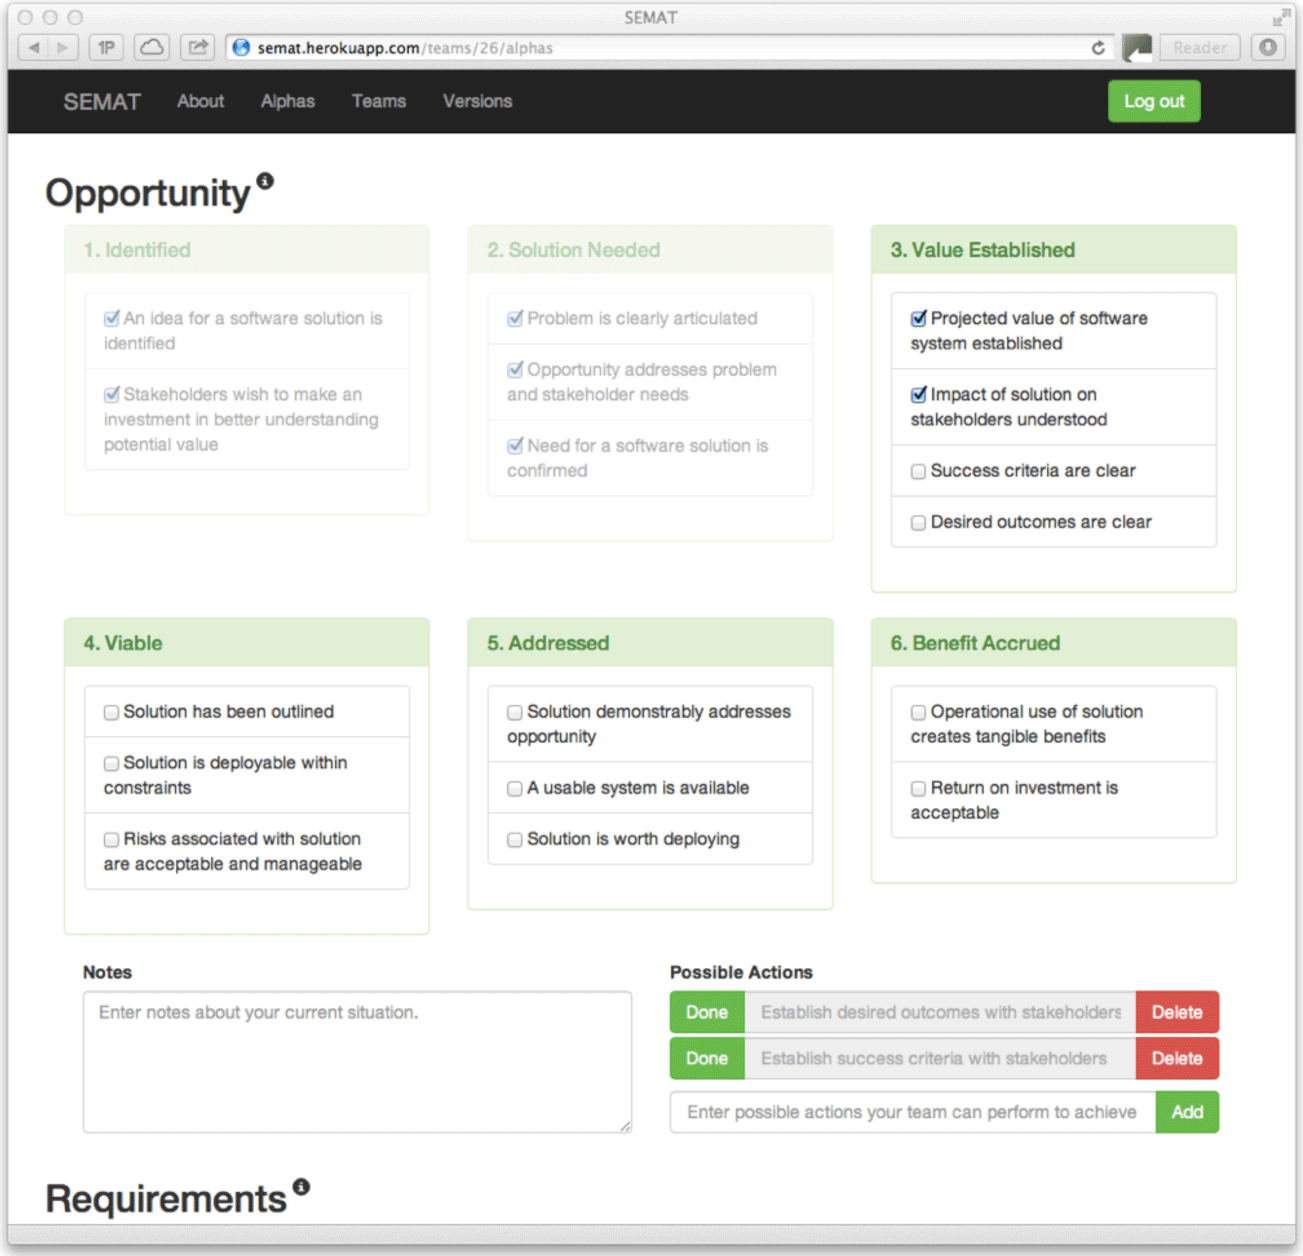
\includegraphics[width=4.00in]{tool_photos/tool_photo}
\caption{Essence Kernel Tool for Essence Reflection Meetings}
\label{EssenceToolScreenshot}
\end{figure}

\begin{figure}[ht]
\centering
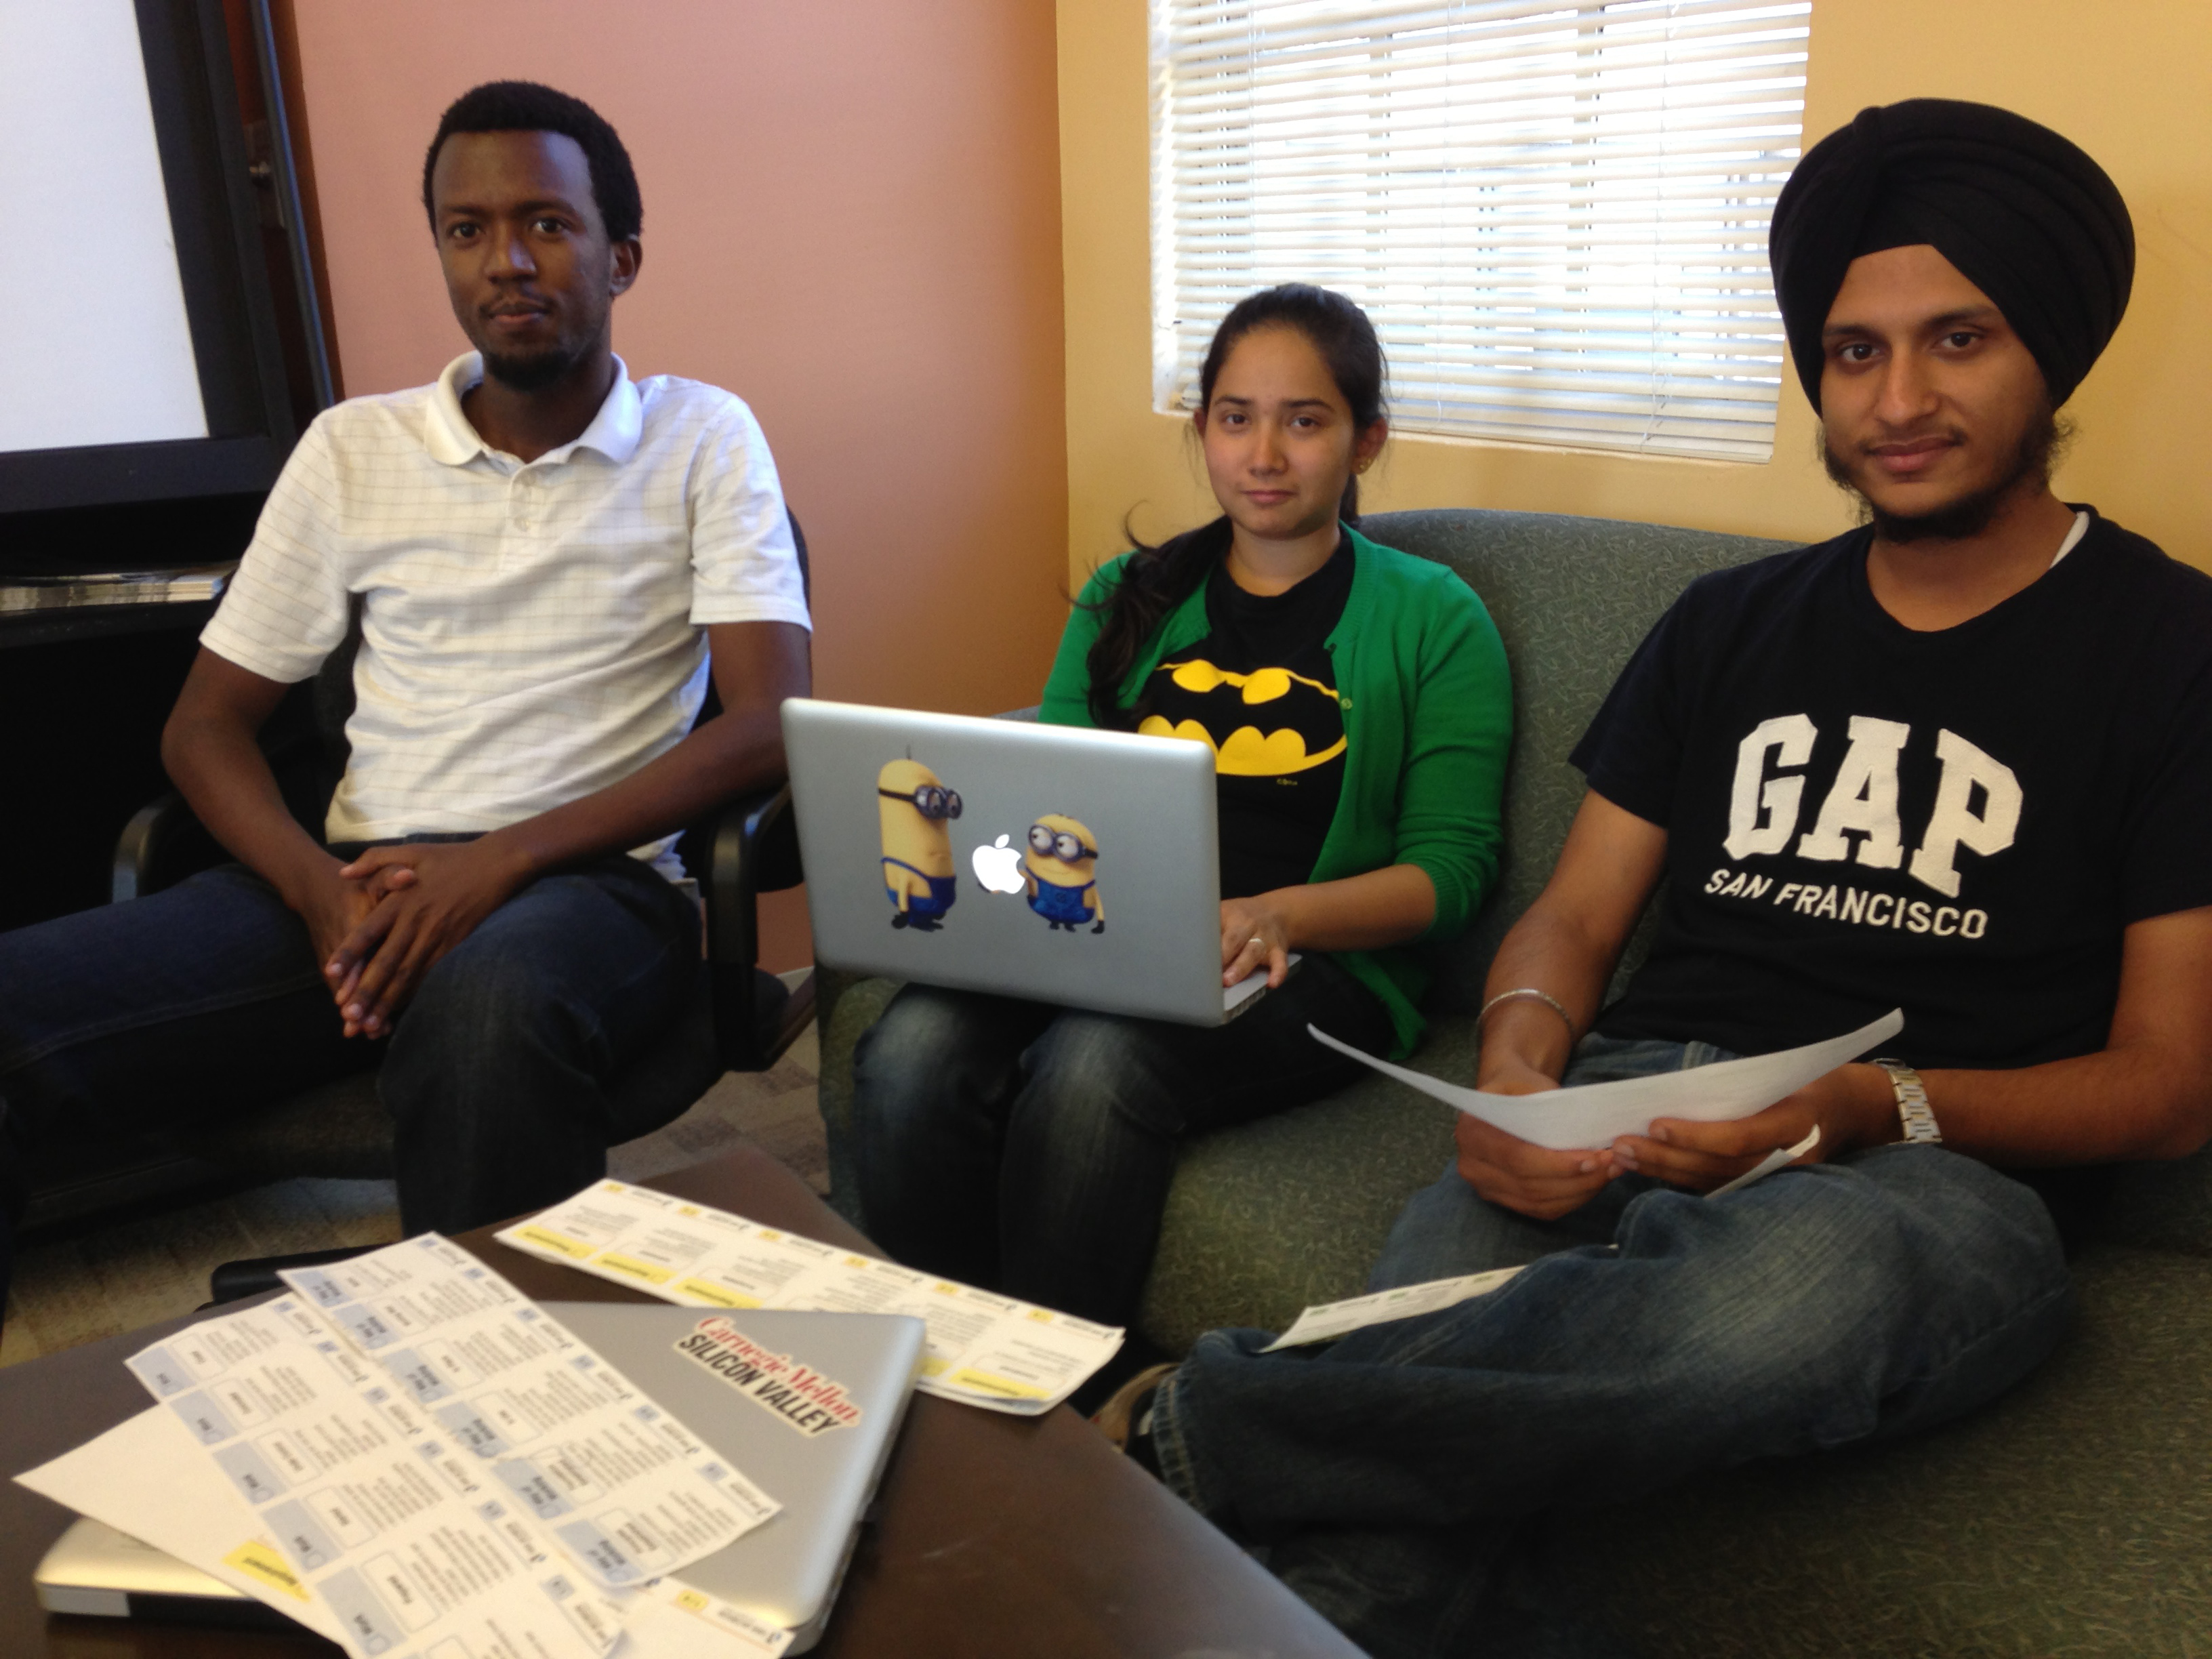
\includegraphics[width=3.00in]{student_photos/team_1}
\caption{Student Team using an Alpha Strip during an Essence Reflection Meeting}
\label{AlphaStrip}
\end{figure}

\subsection{Kernel Support and Tooling}
\label{EssenceTool}
I created a research tool for supporting team-based software development for the purpose of reducing preparation time, increasing the efficiency of Essence Reflection meetings, decreasing training time, and streamlining data collection. A screen-shot of the tool is shown in Figure \ref{EssenceToolScreenshot}. 

\textit{The tool reduces preparation time}: Before the tool existed, I would print the kernel and, using a paper cutter, cut out 42 individual state card for each team member. This was time consuming and laborious.  In the next semester, I printed, on legal paper, seven alpha strips per team member by combining alpha states into one full strip. Figure \ref{AlphaStrip} shows a team using an alpha strip. Printing and cutting continued to be time consuming. The tool minimizes preparation time to simply providing the email addresses of each team member. 

\textit{The tool increases the efficiency of Essence Reflection meetings}: The tool removes the need to handout materials during meetings and the tool helps a team learn the kernel by focusing the team on one alpha at a time. Before handing out sets of 42 cards to each team member was tedious. After switching to the seven alpha strips, distributing them one at a time still resulted in shuffling of paper. For distributed teams I used Google Drawings in Google Documents to draw the alpha state cards, but the slowness and various limitations of the application made for a painful user experience. My tool sequenced the needed information in one logical flow  resulting in just in time learning. Once the team finishes entering their information, a ``done" button emails everyone on the team (including the faculty) the project's current state for each alpha, all captured notes, and a list of work items for the team to accomplish. 

\textit{The tool streamlined data collection}:  Before the tool, the data presentation and data collection were in separate places. The alpha state checklists were presented on a sheet of paper. The data collection was done manually using spreadsheets. The tool places all data in a single location and automates data collection, streamlining the research process.
%Once the semester was over we would convert the Google spreadsheet data into different representations to create graphs indicating team progress through the semester in order to help analyze the data.  

%Prior to the first Essence Reflection meeting, a faculty member log ins in, creates a team, and adds each student member to the team. During the first meeting, one team member shows the first alpha on a projector or TV screen in a conference room.
%I conducted usability testing on the tool and incorporated the feedback into the tool. This enabled me to improve the tool's usefulness and reduce issues for novice users. 

\subsection{Kernel Optimization}
\label{KernelOptimization}
The purpose of this exploratory work was to demonstrate one way to generate a candidate Essence kernel directly from empirical data, not to recommend a replacement for the original Essence kernel \cite{SCSE2015}. 
Using collected empirical data on how teams progress through the Essence kernel during their project, I leveraged genetic algorithms to generate candidate replacement kernels based on that empirical data. 
The genetic program initializes a population with random permutations of the existing kernel and then evolves the population's members by randomly re-arranging checklist items using three different operators. I created the Partial Order fitness function to evaluate how well a candidate kernel explains the empirical data. The fitness function rewards kernels that sequence checklists in the same order that teams accomplish them. 

% \begin{itemize}
% \item ``Move checklist item" operator randomly selects a checklist item and moves it to a different state. If the new state has more than eight checklist items, the code automatically splits that state into two states using the ``split state" operator. The genetic program exercised this operator 80\% of the time.
% \item ``Split state" operator randomly selects a state and subdivides it by creating a new subsequent state and moves half of the checklist items to the new state. The genetic program exercised this operator 10\% of the time.
% \item ``Delete state" operator randomly deletes a state by moving all of its checklist items randomly to other states. The genetic program exercised this operator 10\% of the time.
% \end{itemize}

The generated kernels outscored the original kernel. When the SEMAT community created the Essence kernel, they relied upon human experience and judgment to select the alphas, states, and checklists. Essence is not grounded by empirical data. 

I analyzed the kernel search space and discovered that, in general, kernels utilizing less alphas scored better than kernels utilizing more alphas. A genetic algorithm starting with eight alphas would evolve to use less and less of them, with the best scoring candidate kernel only using one alpha as seen in Figure \ref{NumberOfAlphasPartialOrdering}. During an Essence Reflection meeting, teams need only to consider a handful of next goals when there is a single alpha. Imagine a team meeting with the perfect oracle. Once describing current state, the oracle suggests several possible goals. Creating such an oracle may require a fundamental shift in the data representation of the Essence kernel. 

\begin{figure}[ht]\vspace*{4pt}
\centerline{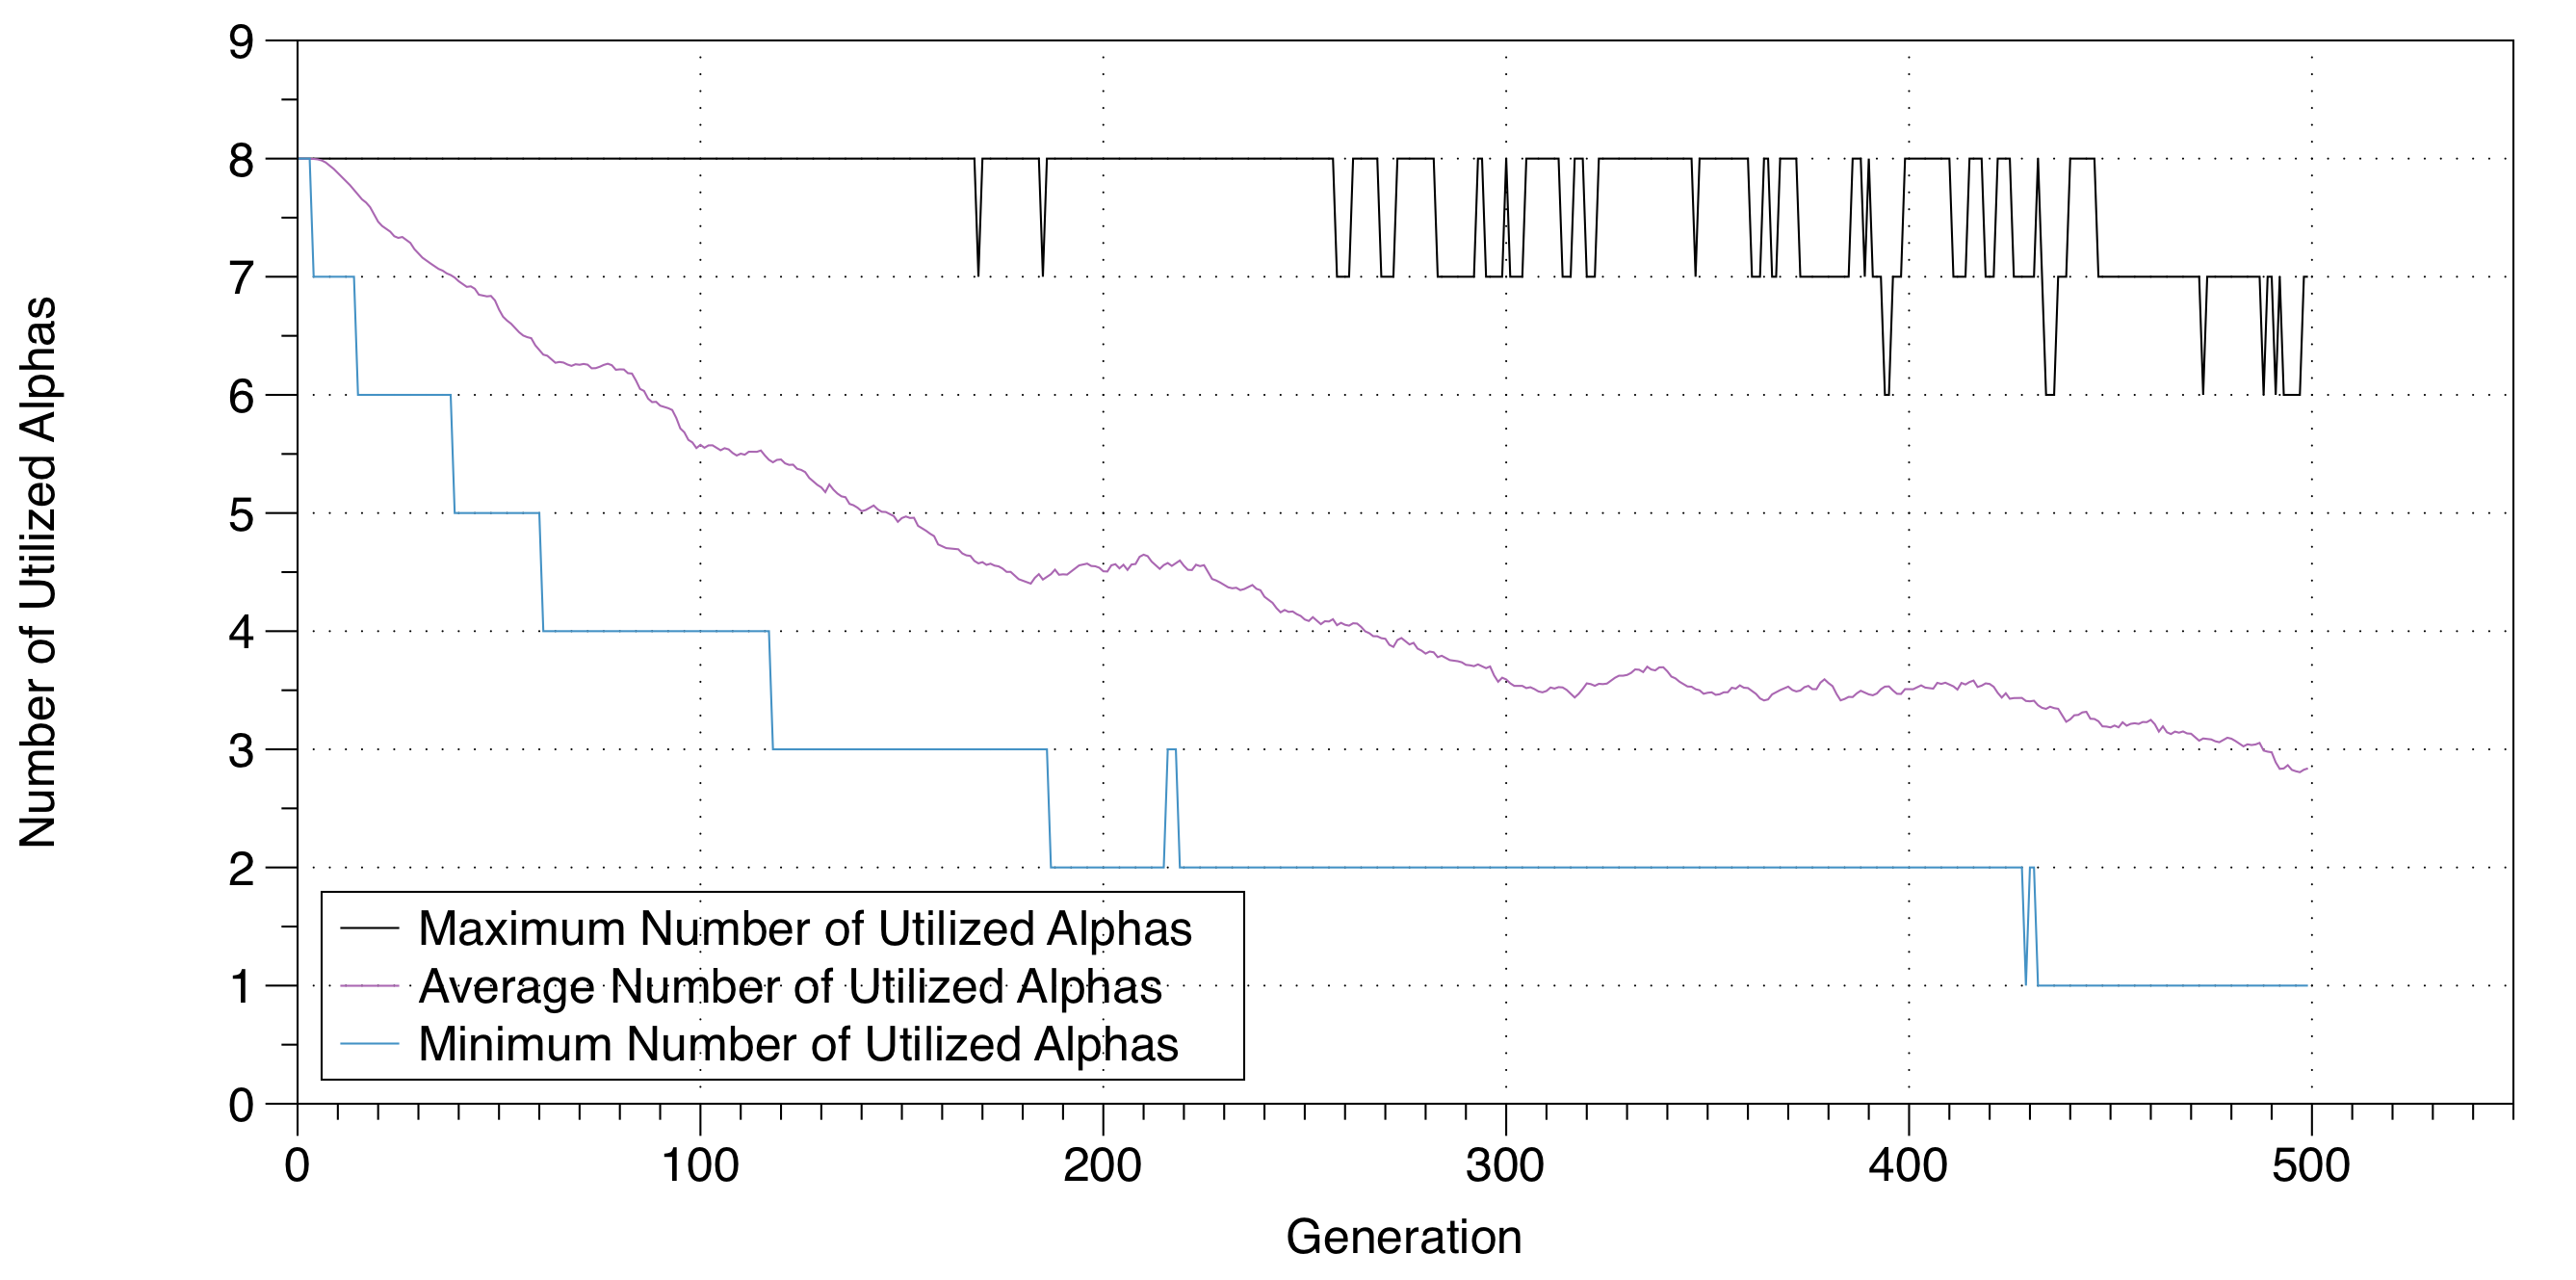
\includegraphics[width=5.00in]{genetic_programming/number_of_alphas_partial_ordering_500gens_40runs_8alpha}}
\caption{Partial Ordering`s Utilization of Number of Alphas}\vspace*{-6pt}
\label{NumberOfAlphasPartialOrdering}
\end{figure}

%While the original kernel appears to be descriptive and the kernel does claim to support any software project, in practice, the kernel is a prescriptive representation. First, the kernel is based on expert experience not directly from project data. Second, when discussing potential modifications to the original kernel based on my project data, the kernel committee (what's the official name?) made comments to the effect of ``that's a nice suggestion, but we don't think that would generalize to all projects" and ``that's a nice suggestion, but I want to represent how projects should be run, not how they are actually run." 

\subsection{Kernel Extension in Industry}
\label{PivotalKernelExtension}
My current research objective is to evaluate the Essence kernel in industry and generate a kernel extension or replacement kernel that models iterative software projects at Pivotal.

To accomplish this objective, I need to answer these research questions:

Research Question 1: Does the kernel support software development as it is done at Pivotal? 

Research Question 2: How would one modify or extend the kernel in order to support iterative development as it is done at Pivotal?

Research Question 3: How does the extension compare to other Essence components such as the Requirements-Item Sub-Alpha and the Software-System Alpha? 

I am using the participant-observer technique by joining software development teams as a full time software engineer. 

In order to understand the Essence's project management and steering approach on industrial projects, I applied the approach to three sequential projects at Pivotal. The collected data confirms that the kernel does not provide value during the construction phase of iterative software in industry, just like what I saw in academia. For quantitative data, I analyzed alpha state progression against earned value from story completion across the duration of a project. For qualitative data, my adviser interviewed me on every aspect of the Essence kernel from a practitioner's point of view. (While self-interview is an accepted practice in this kind of research, we decided it would be better to have an explicit interviewer and interviewee.) After I transcribed this 4.5 hour multiple-day interview, I mined the content for specific issues with applying the Essence kernel on these projects at Pivotal. 

In order to create a kernel replacement, I am using grounded theory to construct a model that accurately reflects empirical data. This iterative research approach allows me to collect data, derive a model from the data, and continue collecting data until the ``saturation'' point when the collection of new data no longer changes the model. As software development occurs, I reflect on the software development experience. Each day I record field study notes briefly describing the accomplishments for my pair and me. Periodically, I analyze the observations to update a draft replacement kernel. New data either support the model or invalidate part of the model. When new data invalidates parts of the model, I will update the model to take into account the new data. In grounded theory, everything is data. I analyzed the team's delivery of 176 stories for a three month project to help further refine the model.

One of the downsides with the participant-observer technique is potential research bias. In order to minimize this issue, I plan to interview Pivotal product managers and Pivotal software engineers. I will record and transcribe these conversations. I will annotate the transcriptions with markers and use these to update the proposed model.

I can achieve these results within the next year. Given my role at Pivotal, I have access to data and resources for software development in industry and thus I am in a unique position for a PhD student.  

% \begin{figure}[h]\vspace*{4pt}
% \caption{Semi-structured Interview Questions}\vspace*{-6pt}\label{InterviewQuestions}
% \begin{itemize}
% \item Please describe your typical day. What is the ``day in the life" of a product manager or software engineer?
% \item What are the characteristics and attributes on an ideal story?
% \item What is the purpose of the iteration planning meeting?
% \item How can you tell if a story is ready for iteration planning meeting and thus ready to be pointed?
% \item What feedback do you get that the project is working well?
% \item Where does usability testing fit into your ideal project?
% \item Please describe your workflow by drawing it on this blank piece of paper.
% \item Please examine this proposed model and critique it.
% \end{itemize}
% \end{figure}

% I plan to interview Pivotal product managers and software engineers until the model stables and the data reaches saturation.

% \subsubsection{Evaluation of Preliminary Results and Implications}
% Note: this section contains representative discussion about the current initial results. The purpose is to illustrate kind of discussion that could happen.

% Figure \ref{KernelExtensionWorkflow} illustrates the state transitions of the \textbf{Story Card} alpha. Pivotal uses story cards in Pivotal Tracker to track and monitor the requirements for a system. The diagram identifies several problems with the kernel's fundamental structure of linear state machines. The normal flow from \textit{Named} to \textit{Accepted} is linear, however, story cards do revert to a previous state. During the Iteration Planning Meeting, stories categorized as \textit{Ready to be Pointed} can be delayed on pointing if the team realizes that the acceptance criteria is not clear, or during the story's discussion, the product manager realizes that there are additional considerations that need to be addressed. \textit{Started} stories often become blocked on dependencies beyond the team's control. \textit{Started} stories sometimes get un-started due to changing project needs. Eventually \textit{Blocked} stories are un-blocked and are ready to be worked on. Once stories are \textit{Delivered}, they can be \textit{Rejected} for a variety of reasons.

% Figure \ref{KernelExtension} shows the checklists for each of these states. The checklists are typical of Essence kernels checklists with two exceptions. The checklists rely on both ``and" and  ``or" conditions to achieve a state. The data collection revealed the tension between prescriptive and descriptive modeling.

% \begin{figure}[ht]
% 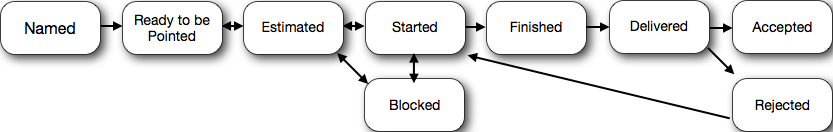
\includegraphics[width=6.25in]{pivotal_images/story_card_workflow}
% \caption{(Initial Results) Pivotal Kernel Extension Workflow Story Card Alpha}
% \label{KernelExtensionWorkflow}
% \end{figure}

% \begin{figure}[ht]
% 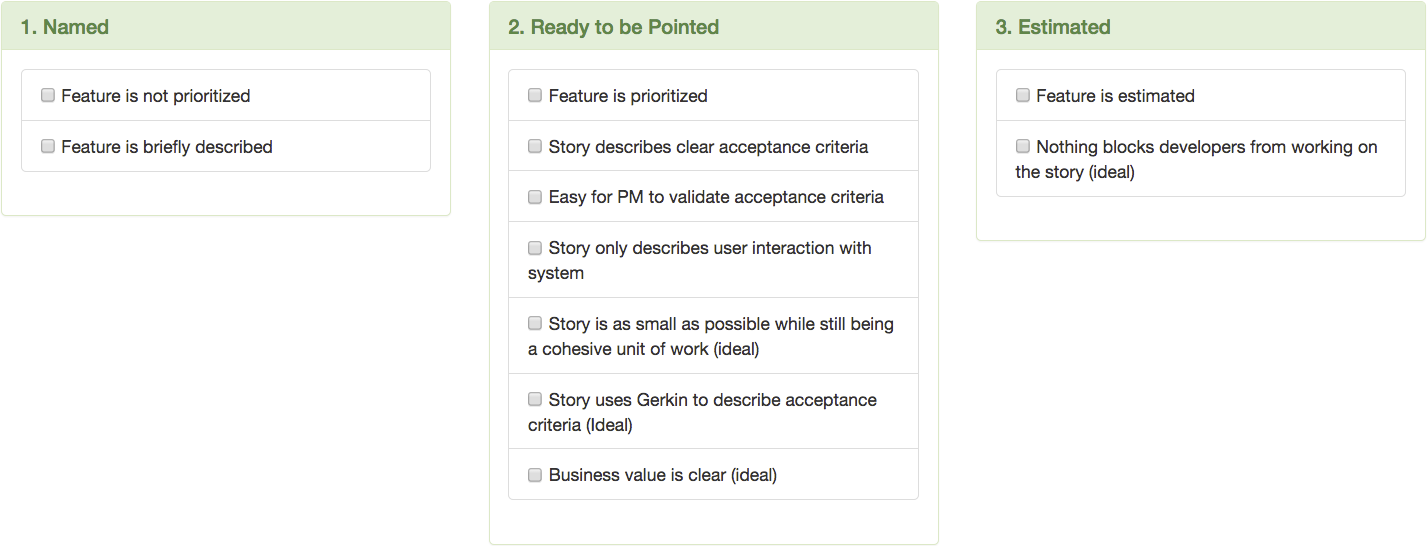
\includegraphics[width=6.25in]{pivotal_images/story_card1}
% 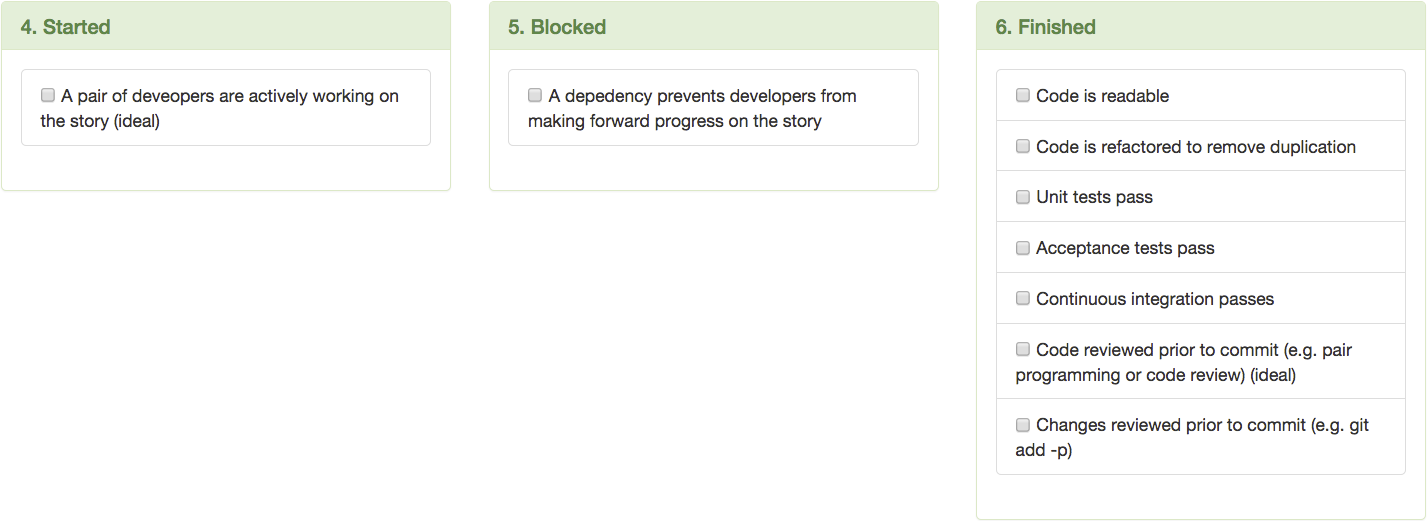
\includegraphics[width=6.25in]{pivotal_images/story_card2}
% 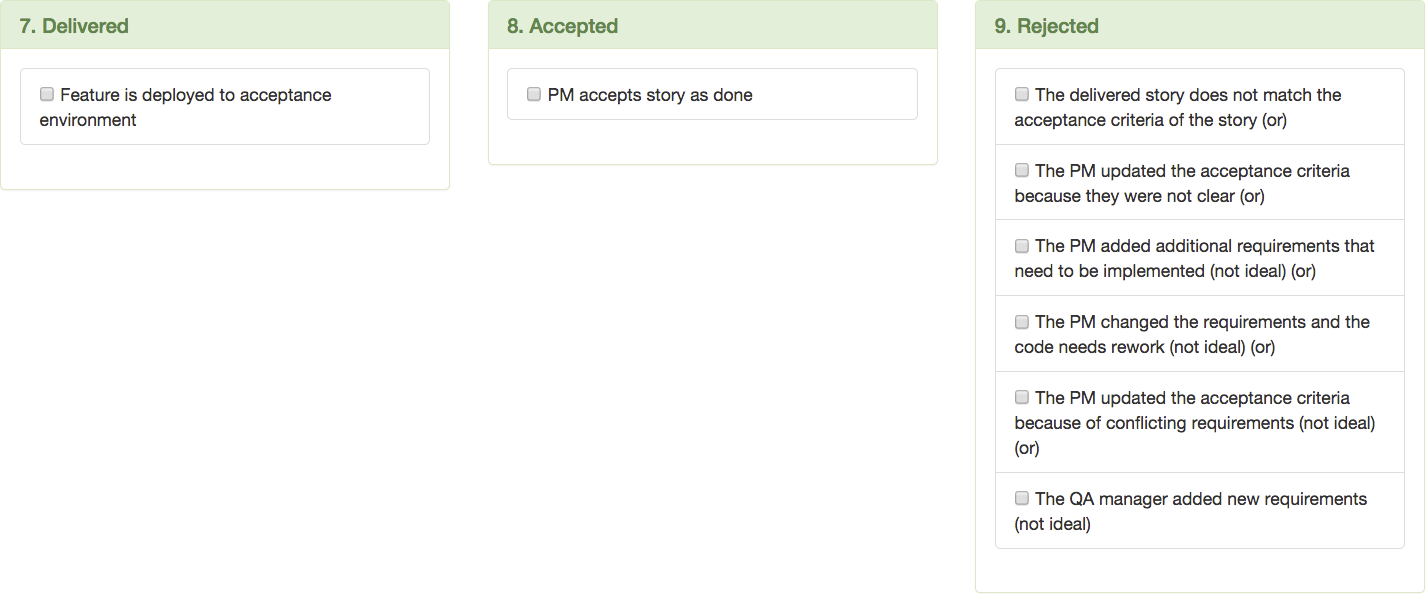
\includegraphics[width=6.25in]{pivotal_images/story_card3}
% \caption{(Initial Results) Pivotal Kernel Extension for Story Card Alpha}
% \label{KernelExtension}
% \end{figure}

% \subsubsection{Necessary modifications to the Essence structure}

% The \textit{Rejected} state happens for a specific reason, thus achieving \textit{any} one of the checklist items causes the state to be achieved and the story to be \textit{Rejected}. The kernel would need a fundamental shift to support this since its underlying language requires accomplishing \textit{all} checklists. 

% Two possible workarounds lose important details and are unappealing. Someone on the kernel author committee might suggest this situation be resolved by replacing the many checklists with a single ``the work is rejected" checklist. This path is unappealing as the proposed checklist both looses interesting information by dumbing-down the model, and simplifies the information into a trivial checklist that is redundant with the state's title. Another possible solution is to collapse the many checklists into a single statement that says ``A or B or C or D" as in ``the delivered story does not match the acceptance criteria of the story OR the PM updated ... OR the PM added ... OR the PM changed ... OR the PM." This run-on sentence makes the checklist difficult to read and understand. 

% There are typical and common reasons for a story to be rejected, two of which fit Pivotal's accepted flows for the work. This raised the issue about whether the kernel should be prescriptive and explain the ``way things should be" or descriptive and explain the ``way things are."

\section{Conclusion}
\label{Conclusions}

% \subsection{Summary}
The SEMAT community created Essence to ``re-found software engineering as a rigorous discipline." The Essence kernel serves as its foundation. The creators claim that it provides support and value to any software engineering project. Several authors have published papers explaining and promoting the Essence kernel. Currently anecdotal evidence indicates that the Essence kernel might add value for software projects. 

My published field study of software development teams in academia revealed that student teams working within the confines of a semester length course realize value in applying the Essence kernel. During Essence Reflection meetings, student teams using the Essence kernel found value during project inception and found less value during the construction phase of iterative  projects. For them, the ratio of project setup to construction enables them to still appreciate the Essence kernel even during weeks in which the kernel provides little guidance. However, on an industry project where project setup is a small piece of the overall project, changes are necessary for the team to realize value from the Essence kernel.

Since most of agile software projects are iterative software development, adapting Essence kernel would increase its potential value to software development teams and the broader SEMAT community. A kernel extension for iterative software development would enable teams to find value from Essence during the construction phase of a project. Given the differences between traditional and iterative software development, possibly two essence kernels would emerge tailored to the unique circumstances of traditional and agile software development.

\appendix
\section{Research Timeline}
\label{appendix}

\begin{table}[H]
\caption{Research Timeline}
\label{ResearchTimeline}
\centering
%\begin{tabular}{|l|l|}
\begin{tabular}{|p{1.00in}|p{5.00in}|}
\hline
Semester    & Activities and Results  \\ \hline
Spring 2013 & Research: Setup for field study \\
            & Research: Facilitated Essence Reflection meetings and collected data for 4 master of software engineering teams. \\ \hline
Summer 2013 & Research: Facilitated Essence Reflection meetings and collected data for 3 master of software engineering teams.  \\ \hline
Fall 2013   & Research: Facilitated Essence Reflection meetings and collected data for 11 master of software engineering teams.  \\ \hline
Spring 2014 & Research: Facilitated Essence Reflection meetings and collected data for 2 master of software engineering teams.\\ 
            & Phd: Passed the ECE PhD qualifier.\\ 
            & Paper: Essence Reflection Meetings: Field Study, EASE 2014. \cite{EASE2014} \\ \hline
Summer 2014 & Research: Facilitated Essence Reflection meetings and collected data for 3 master of software engineering teams.\\ 
            & Paper: State-based Monitoring and Goal-driven Project Steering: Field Study of the SEMAT Essence Framework, ICSE 2014. \cite{ICSE2014} \\ \hline
Fall 2014   & Research: Setup for field study \\
            & Research: Collected data from Participant-Observation on two projects at Pivotal Labs.  \\ \hline
Spring 2015 & Research: Collected data from Participant-Observation on one project at Pivotal Labs.\\ 
            & Paper: Towards Generating Essence Kernels Using Genetic Algorithms, SCSE 2015. \cite{SCSE2015} \\ 
            & Tutorial: Using Essence Reflection Meetings in Team-Based Project Courses, SCSE 2015.\cite{SCSE2015Tutorial} \\ \hline
Summer 2015 & Research: Kernel extension for iterative software projects.\\ 
            & Workshop: Essence in Team-Based Project Courses, CSEE\&T 2015. \cite{CSEET2015Workshop} \\ \hline                     
\end{tabular}
\end{table}

%% References
%%
%% Following citation commands can be used in the body text:
%% Usage of \cite is as follows:
%%   \cite{key}         ==>>  [#]
%%   \cite[chap. 2]{key} ==>> [#, chap. 2]
%%

%% References with bibTeX database:

\bibliographystyle{elsarticle-num}
% \bibliographystyle{elsarticle-harv}
% \bibliographystyle{elsarticle-num-names}
% \bibliographystyle{model1a-num-names}
% \bibliographystyle{model1b-num-names}
% \bibliographystyle{model1c-num-names}
% \bibliographystyle{model1-num-names}
% \bibliographystyle{model2-names}
% \bibliographystyle{model3a-num-names}
% \bibliographystyle{model3-num-names}
% \bibliographystyle{model4-names}
% \bibliographystyle{model5-names}
% \bibliographystyle{model6-num-names}

\bibliography{bibliography}


\end{document}

%%
%% End of file `elsarticle-template-num.tex'.




% "The checklists of an alpha state are joined by AND. The state of an alpha is deemed to be the most advanced (favourable) state for which all checklists are true." (OMG standard)

% "The checklists of a work product level of detail are joined by OR. The level of detail of a work product is deemed to be the most detailed level for which at least one checklist is true." (OMG standard)

fullfilledSuccessorLevel: my_LevelOfDetail 􏰃 my_LevelOfDetail fullfilledSuccessorLevel (l) =
if (l.successor = 􏰌) {l}
else
let mc = {c | c 􏰆 s.successor.checkpoints 􏰊 not c.isFullfilled} in (if (mc = 􏰌) {fullfilledSuccessor(s.successor)} else {l})


derive_current_state: my_Alpha 􏰃 my_State
derive_current_state (a) =
lets={s|s 􏰆 a.states 􏰊 {ps|ps.successor=s}= 􏰌} in fullfilledSuccessorState(s)